%%%%%%%%%%%%%%%%%%%%%%%%%%%%%%%%%%%%%%%%%%%%%%%%%%%%%%%%%%%%%%%%%%%%%%
%%                     Or
%%%%%%%%%%%%%%%%%%%%%%%%%%%%%%%%%%%%%%%%%%%%%%%%%%%%%%%%%%%%%%%%%%%%%%
%\color{blue}
\subsection{Glyph: \glyph{Or}}\label{sec:or}

\begin{description}
 \item[SBO]\mbox{}\\ SBO:0000174 ! or.
 \item[origin]\mbox{}\\ More than one EPN (section~\ref{sec:EPNs}) or logical operator (section~\ref{sec:logic}).
 \item[target]\mbox{}\\  One modulation (section~\ref{sec:modulation}), stimulation (section~\ref{sec:stimulation}), catalysis (section~\ref{sec:catalysis}), inhibition (section~\ref{sec:inhibition}) or trigger (section~\ref{sec:trigger}) arcs.
 \item[node]\mbox{}\\ \glyph{or} is represented by a circle carrying the word ``or''.
 \end{description}

\begin{figure}[H]
  \centering
  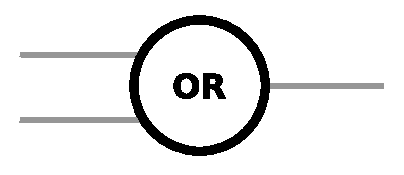
\includegraphics[scale = 0.5]{images/or}
  \caption{The \PD glyph for \glyph{or}.}
  \label{fig:or}
\end{figure}


